\documentclass[t]{beamer}
\usecolortheme[RGB={0,114,197}]{structure} 
\usetheme{Ilmenau} 
\usepackage{tikz}
\usepackage{multicol}

\title{Software-Ontwerp}
\subtitle{Iteratie 2}
\author{Reniers V. - Devlieghere J. - Castel D. - Pante S.}
\institute{KU Leuven}

\begin{document}

\frame{\titlepage} 
\begin{frame}{Inhoud}
\begin{multicols}{2}
\tableofcontents
\end{multicols}
\end{frame}



\section{Inleiding} 
\begin{frame}{Inleiding} 
Thema's die aan bod komen:
\begin{itemize}
	\item High-Level bespreking van het ontwerp.
	\item Onderdelen in detail bekeken.
	\item GRASP en design patterns.
	\item Uitbreidbaarheid van het ontwerp.
	\item Test cases.
\end{itemize}
\end{frame}

\subsection{Rolverdeling}
\begin{frame}{Rolverdeling}
\begin{multicols}{2}
\tableofcontents[currentsection]
\end{multicols}
\end{frame}

\begin{frame}{Rolverdeling}
Iteratie 2:
\begin{itemize}
	\item Lead Designer: Jonas Devlieghere
	\item Lead Tester: Vincent Reniers
\end{itemize}

Iteratie 3:
\begin{itemize}
	\item Lead Designer: Dieter Castel
	\item Lead Tester: Stefan Pante
	\item Domain Modeler: Vincent Reniers
\end{itemize}
\end{frame}

\subsection{Werkverdeling}

\begin{frame}{Werkverdeling}
Iteratie 2: 1 maart - 15 maart

\begin{center}
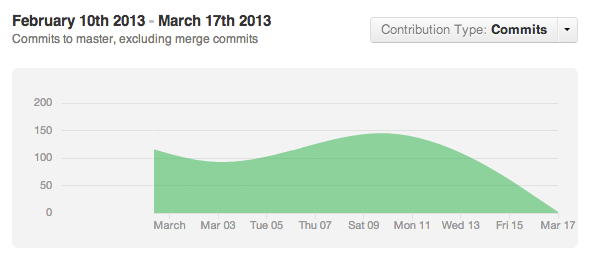
\includegraphics[width= 0.90\linewidth]{images/flowchart}
\end{center}

Uren gepresteerd: 45 uur per persoon.

\end{frame}
\section{Het ontwerp}
\subsection{Basisstructuur}
\begin{frame}{Basisstructuur}
\begin{multicols}{2}
\tableofcontents[currentsection]
\end{multicols}
\end{frame}


\begin{frame}{Besluit}
\vspace{0.8in}
\begin{center}
Bedankt voor uw aandacht.
\end{center}
\end{frame}

\end{document}
